\documentclass[12pt]{article}

\usepackage[dvips,letterpaper,landscape]{geometry}
\usepackage[pdftex]{graphicx}
\usepackage{afterpage}
% \special{landscape}
% \usepackage[letterpaper,landscape]{geometry}

\textheight 6.5in

%opening
\title{Dynamic Air Trapping vs. Emphysema Analysis }
\date{}
% \author{}

\begin{document}

\maketitle

The aeroted lung image is obtained by segmenting the inspiration image below threshold -50 HU (noted as \textbf{\textit{aeroted}} below). The emphysema area is obtained by segmenting below the inspiration image below threshold -910 HU (noted as ``\textbf{\textit{severe}}'' below). The dynamic air trapping area is obtained by segmenting the non-severe and aeroted lung difference image with variant thresholds (noted as ``\textbf{\textit{dyn}}'' below). We choose threshold from 0 to 200 in every 25 HU.

For each threshold, we compute the following ratios:
\begin{enumerate}
 \item severe / aeroted
 \item dyn / aeroted
 \item dyn+severe /aeroted
\end{enumerate}

The following images show the correlation value between these raiots and PFT values. X-axis is PFT and Y-axis is ratios annoted with the correspoind threshold. For example, ``dyn 50'' means the ratio for dyn / aeroted with threshold = 50.



\begin{figure}
    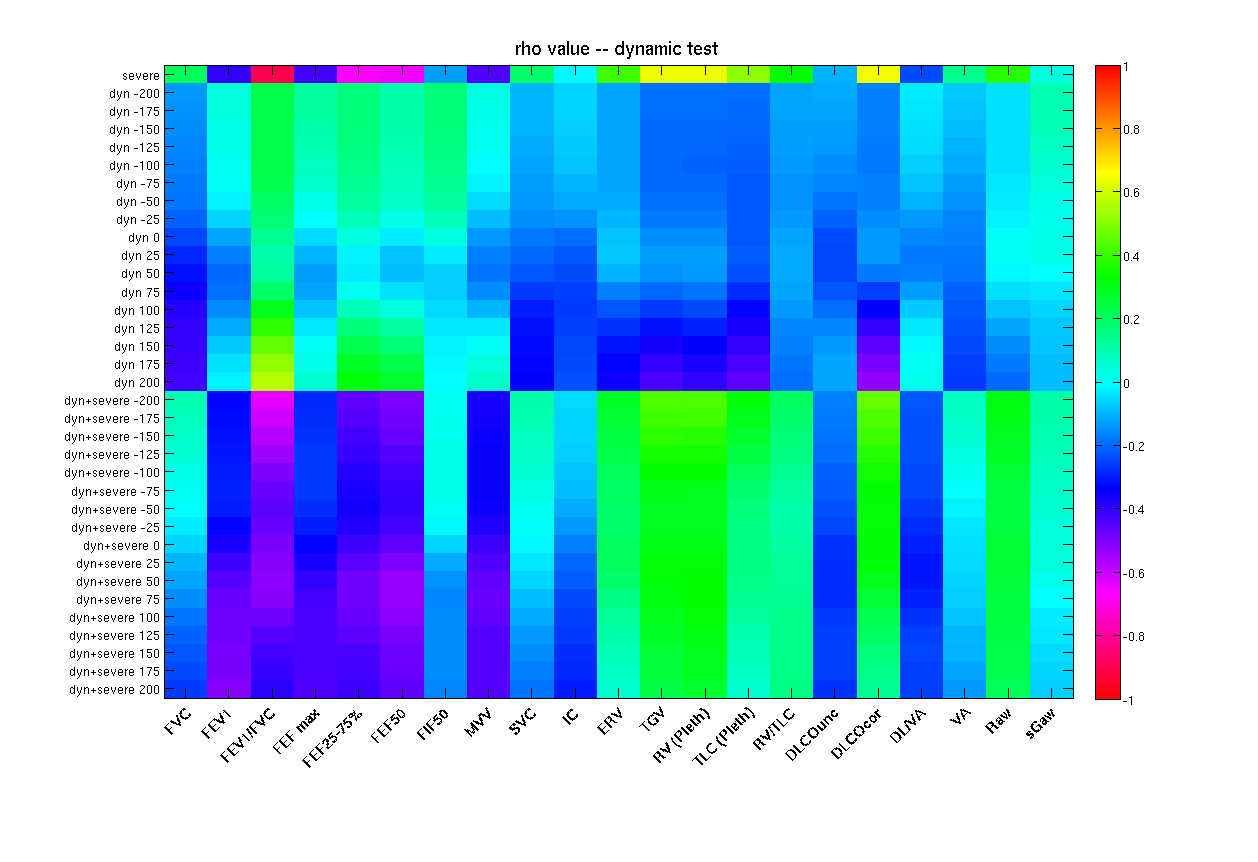
\includegraphics[width=0.84\linewidth,viewport=100 60 720 550]{dyn/rho_dyn.png}
    \caption{rho value for different ratios vs PFT, on the whole database. X axis is PFT. Y axis is computed ratios. The number of Y axis label is the corresponding threshold chosen for segmenting dynamic air trapping area.}
    \label{fig:rho-ILD----metrics-vs-PFT----Whole-Lung-Expiration}
\end{figure}
\begin{figure}
    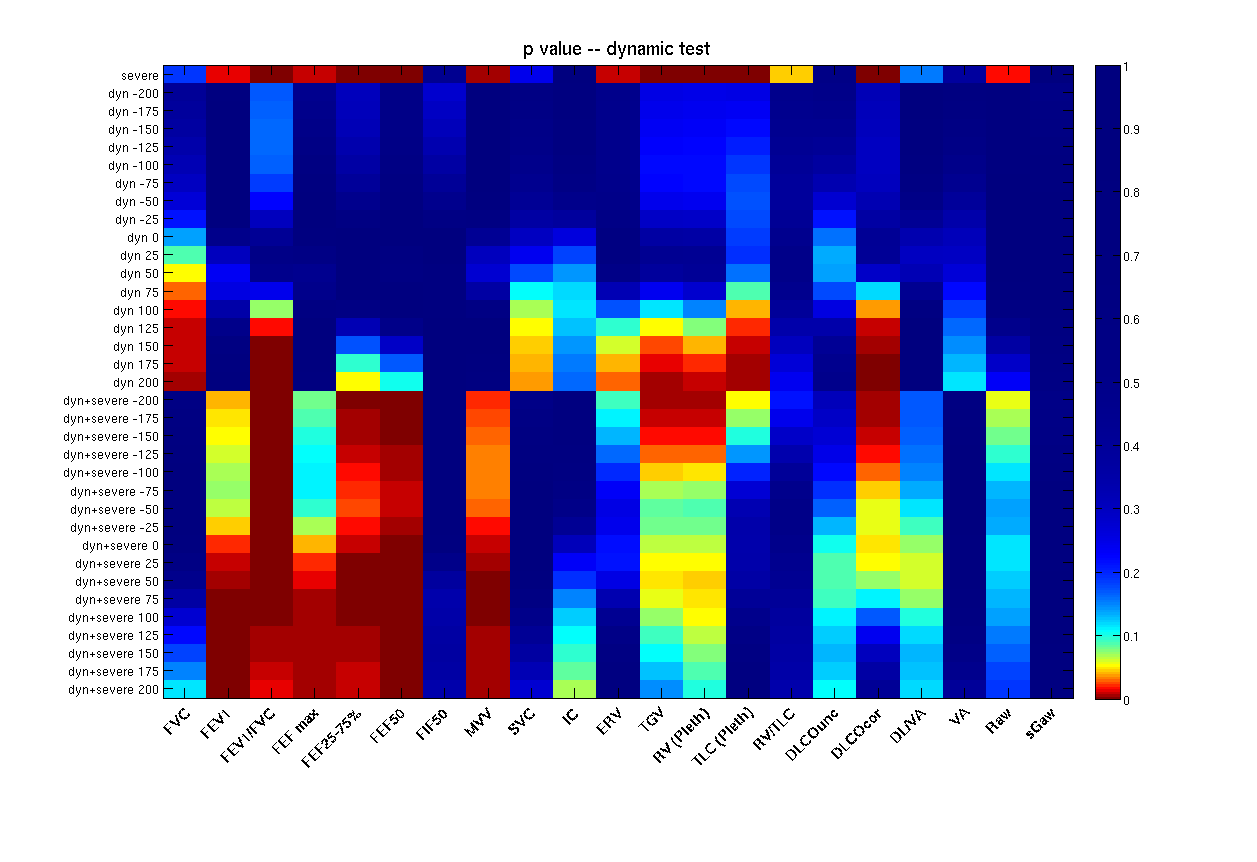
\includegraphics[width=0.84\linewidth,viewport=100 60 720 550]{dyn/p_dyn.png}
    \caption{p value for different ratios vs PFT, on the whole database. X axis is PFT. Y axis is computed ratios. The number of Y axis label is the corresponding threshold chosen for segmenting dynamic air trapping area.}
    \label{fig:p-ILD----metrics-vs-PFT----Whole-Lung-Expiration}
\end{figure}

% Another illustration is to see if the computed ratios can differiate ILD from COPD cases. The following shows the best correlation case for ? and threshold = ?. The left shows ILD data and right shows COPD data. 

% \begin{figure}
%     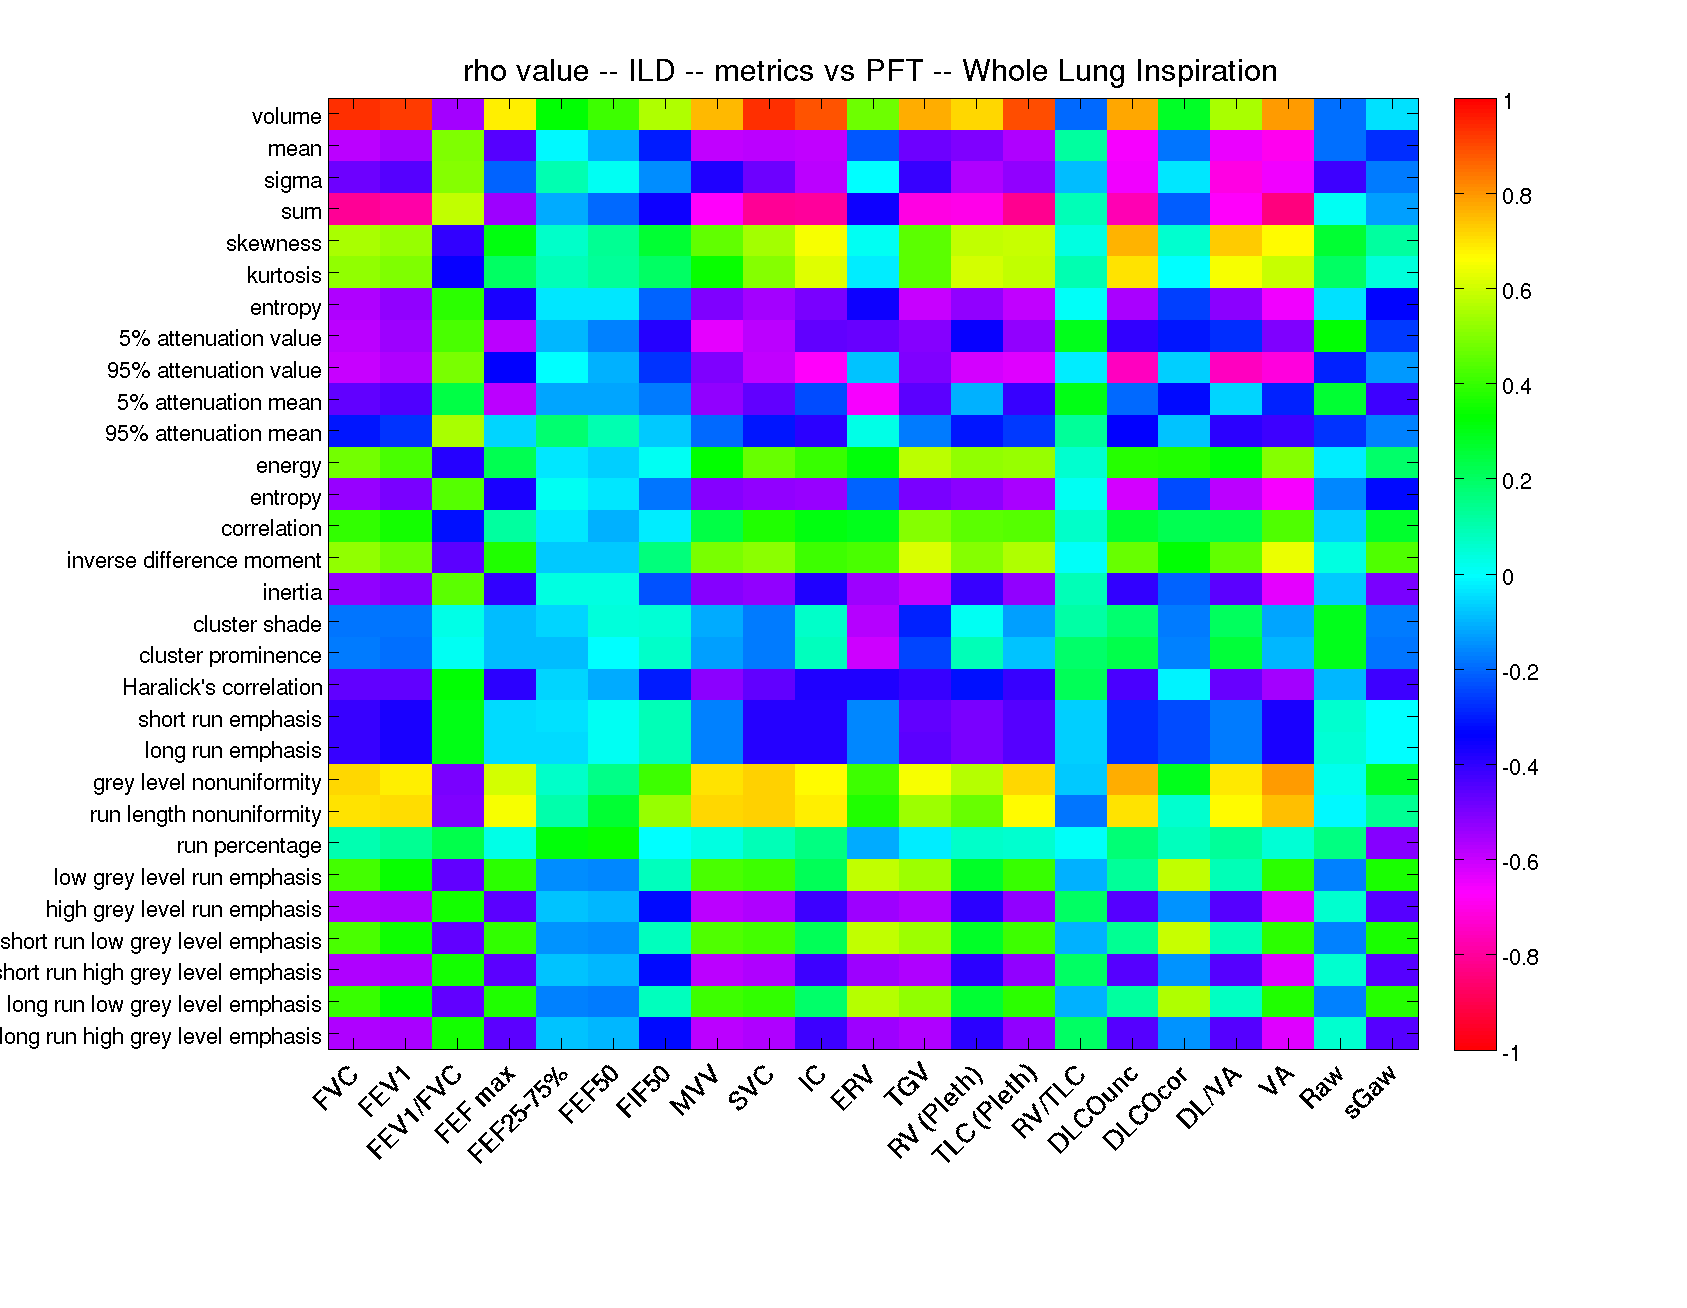
\includegraphics[width=0.84\linewidth,viewport=100 60 620 550]{corr/rho-ILD----metrics-vs-PFT----Whole-Lung-Inspiration.png}
%     \caption{Best correlated ratio values. The left shows the values for ILD data and right shows the values for COPD data.}
%     \label{fig:rho-ILD----metrics-vs-PFT----Whole-Lung-Inspiration}
% \end{figure}


\end{document}
